\documentclass{oblivoir}
\usepackage{amsmath,amssymb,amsthm,kotex,mdframed,paralist,kswrapfig}

\newcounter{num}
\newcommand{\prob}
{\bigskip\noindent\refstepcounter{num}\textbf{문제 \arabic{num})}\par}

\newcommand{\ans}{{\raggedleft\textbf{답 : (\qquad\qquad\qquad\qquad\qquad\qquad)}
\par}\bigskip\bigskip}


%%%
\begin{document}
\Large

\title{승재 11 - 6학년 2학기 - 04}
\author{}
\date{\today}
\maketitle
%\tableofcontents

\newpage

%
\prob
민희와 효연이는 공부를 하다가 사과 두 개를 먹었습니다.
첫 번째 사과는 반으로 나누었는데 민희는 그 중 한 조각을 먹었고
두 번째 사과는 3조각으로 나누었는데 민희는 이번에도 한 조각을 먹었습니다.
그리고 나머지 사과는 모두 효연이가 먹었습니다.
민희와 효연이가 먹은 사과의 양을 가장 간단한 자연수의 비로 나타내세요.

\ans

\begin{figure}[h!]
\centering
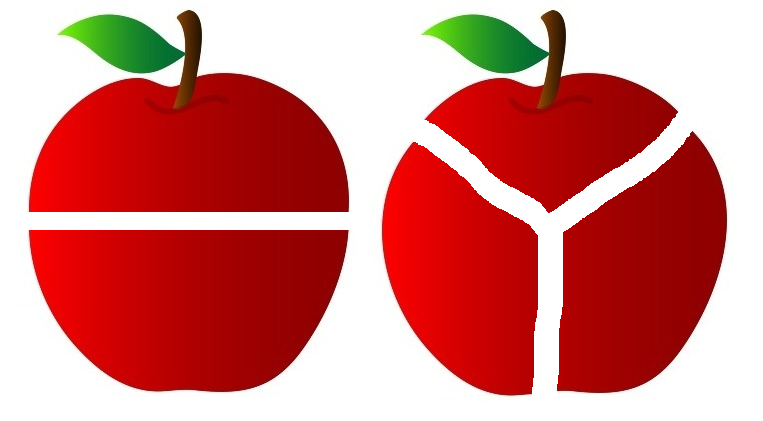
\includegraphics[width=0.6\textwidth]{01-1}

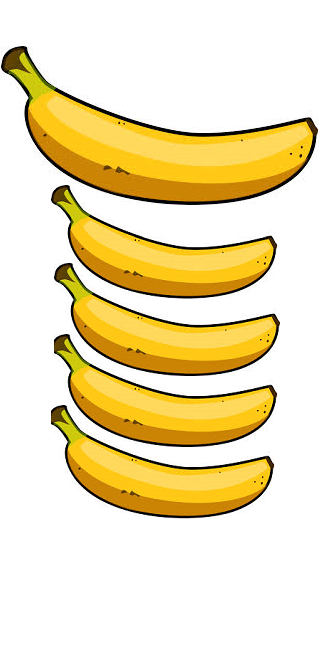
\includegraphics[width=0.6\textwidth]{01-2}

민희가 먹은 사과

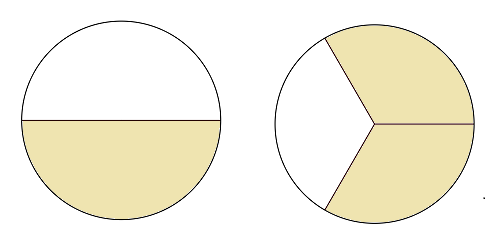
\includegraphics[width=0.6\textwidth]{01-3}

효연이가 먹은 사과
\end{figure}

\newpage

%
\prob
지호와 영신이는 공부를 하다가 사과 두 개를 먹었습니다.
첫 번째 사과는 4등분을 하였는데 지호는 그 중 3조각을 먹었고
두 번째 사과는 8등분을 하였는데 지호는 그 중 5조각을 먹었습니다.
그리고 나머지 사과는 모두 영신이가 먹었습니다.
지호와 영신이가 먹은 사과의 양을 가장 간단한 자연수의 비로 나타내세요.

\ans

\begin{figure}[h!]
\centering
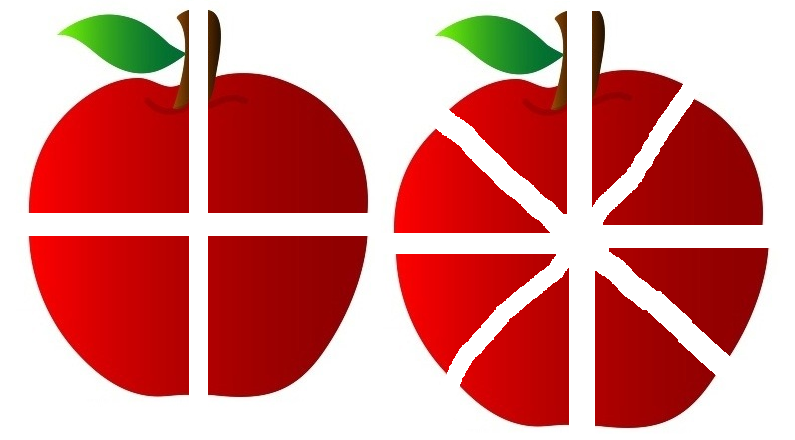
\includegraphics[width=0.6\textwidth]{02-1}

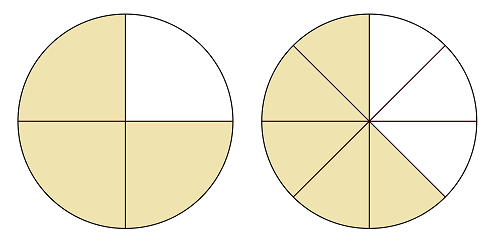
\includegraphics[width=0.6\textwidth]{02-2}

지호가 먹은 사과

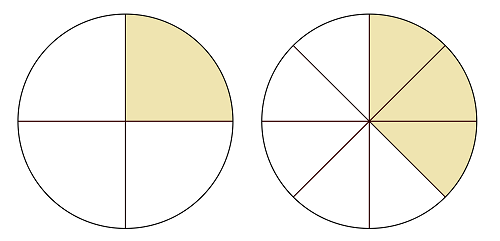
\includegraphics[width=0.6\textwidth]{02-3}

영신이가 먹은 사과
\end{figure}

\newpage

%
\prob
지수와 효정이는 공부를 하다가 사과 두 개를 먹었습니다.
첫 번째 사과는 8등분을 하였는데 지수는 그 중 세 조각을 먹었고
두 번째 사과는 10등분을 하였는데 지수는 그 중 일곱 조각을 먹었습니다.
그리고 나머지는 효정이가 모두 먹었습니다.
지수와 효정이가 먹은 사과의 양을 가장 간단한 자연수의 비로 나타내세요.

\ans

\begin{figure}[h!]
\centering
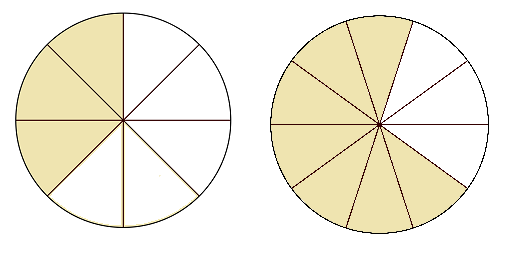
\includegraphics[width=0.7\textwidth]{03-1}

지수가 먹은 사과

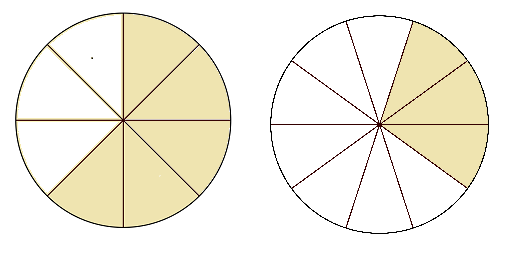
\includegraphics[width=0.7\textwidth]{03-2}

효정이가 먹은 사과
\end{figure}

\newpage

%
\prob
윤지와 준호는 사과 세 개를 먹었습니다.
첫 번째 사과는 6등분했는데 모두 윤지가 먹고, 두 번째 사과는 8등분했는데 모두 준호가 먹었습니다.
세 번째 사과는 7등분하여 3조각을 윤지가 먹고 4조각을 준호가 먹었습니다.
윤지와 준호가 먹은 사과의 양을 가장 간단한 자연수의 비로 나타내세요.

\begin{figure}[h!]
\centering
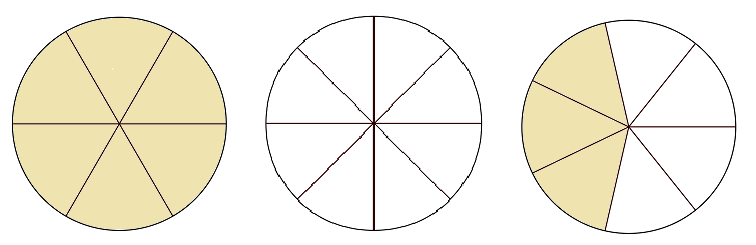
\includegraphics[width=0.7\textwidth]{04-1}

윤지가 먹은 사과

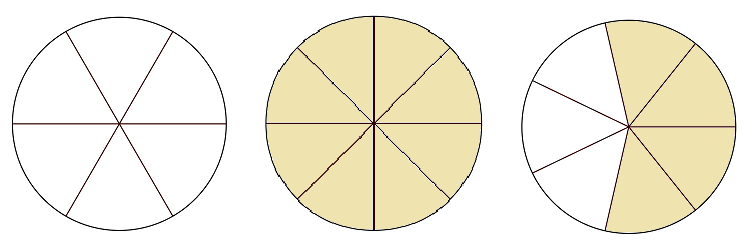
\includegraphics[width=0.7\textwidth]{04-2}

준호가 먹은 사과
\end{figure}

\ans

\newpage

%
\prob
다음은 한 변의 길이가 1cm인 쌓기나무를 사용하여 수를 나타낸 것입니다.

\begin{figure}[h!]
\centering
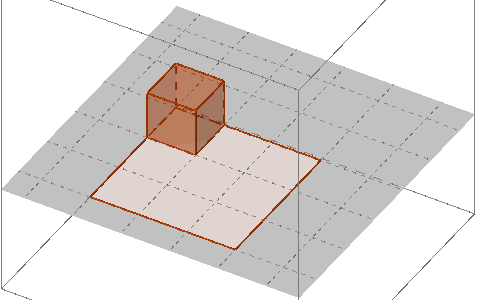
\includegraphics[width=0.45\textwidth]{05-001}
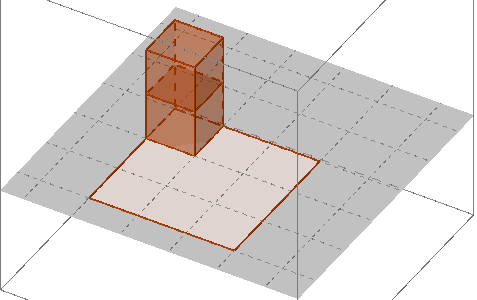
\includegraphics[width=0.45\textwidth]{05-002}

1\qquad\qquad\qquad\qquad\qquad\qquad\qquad\qquad2
\bigskip

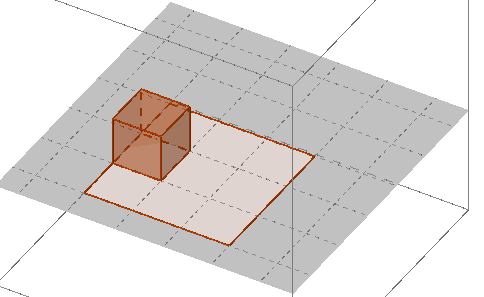
\includegraphics[width=0.45\textwidth]{05-003}
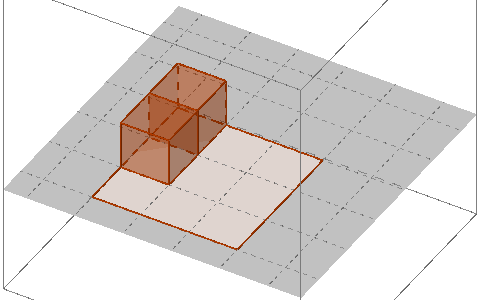
\includegraphics[width=0.45\textwidth]{05-004}

3\qquad\qquad\qquad\qquad\qquad\qquad\qquad\qquad4
\bigskip

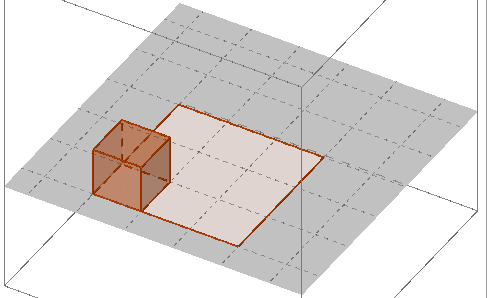
\includegraphics[width=0.45\textwidth]{05-009}
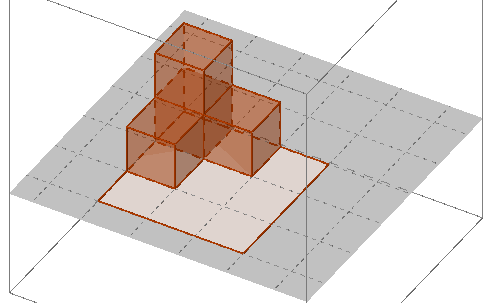
\includegraphics[width=0.45\textwidth]{05-015}

9\qquad\qquad\qquad\qquad\qquad\qquad\qquad\qquad15
\bigskip

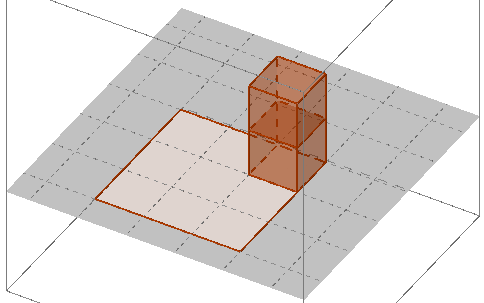
\includegraphics[width=0.45\textwidth]{05-200}
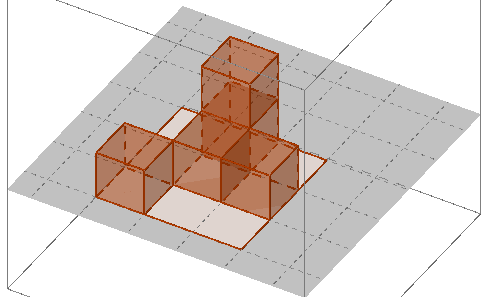
\includegraphics[width=0.45\textwidth]{05-359}

200\qquad\qquad\qquad\qquad\qquad\qquad\qquad\qquad359
\end{figure}
\newpage

(1) 다음 도형들이 나타내는 수를 구하세요.

\begin{figure}[h!]
\centering
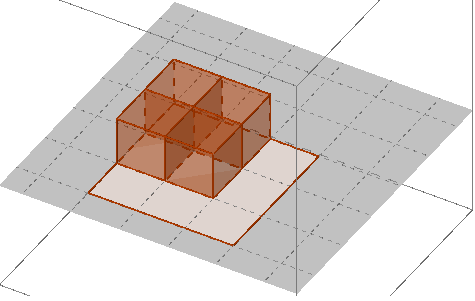
\includegraphics[width=0.45\textwidth]{05-044}
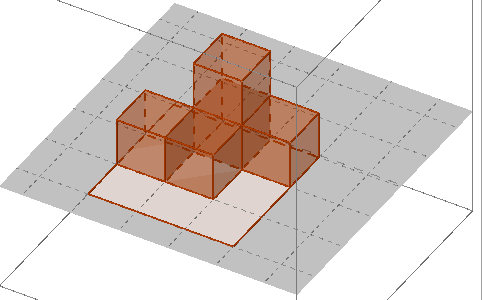
\includegraphics[width=0.45\textwidth]{05-153}

(\qquad\qquad\qquad)\qquad\qquad\qquad\qquad\qquad(\qquad\qquad\qquad)
\bigskip\bigskip

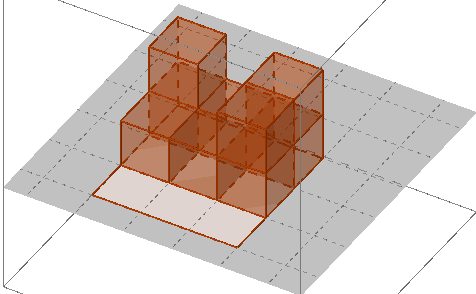
\includegraphics[width=0.45\textwidth]{05-845}
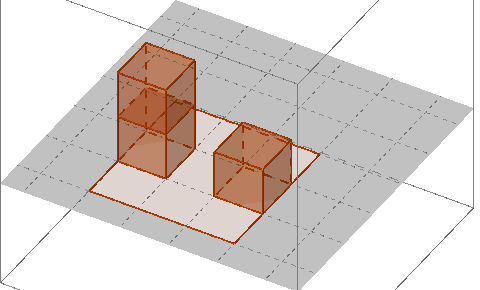
\includegraphics[width=0.45\textwidth]{05-306}

(\qquad\qquad\qquad)\qquad\qquad\qquad\qquad\qquad(\qquad\qquad\qquad)
\end{figure}

(2) 45가 나타내는 도형에는 쌓기나무가 몇 개 사용됩니까?

\ans

(3) 263이 나타내는 도형에는 쌓기나무가 몇 개 사용됩니까?

\ans

(4) 17이 나타내는 도형의 겉넓이를 구하세요.

\ans

(5) 729가 나타내는 도형의 겉넓이를 구하세요.

\ans


\newpage

\prob
\kswrapfig[Pos=r]{snail_02}{
오른쪽 그림은 달팽이집을 자세히 관찰한 것입니다.
민희는 달팽이집의 모양을 자세히 그려보았더니 아래 그림과 같이 생긴 모양처럼 그려진다는 것을 알아냈습니다.}

\begin{figure}[h!]
\centering
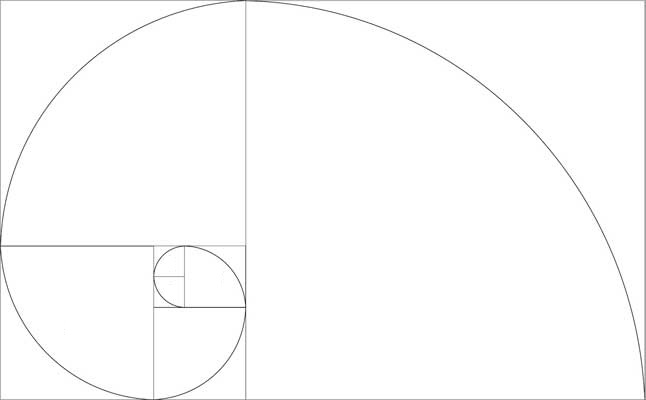
\includegraphics[width=0.9\textwidth]{fibonacci_05}
\end{figure}

이 그림에 나타나는 사각형은 모두 정사각형이고 굽은 선은 원의 일부입니다.
가장 작은 정사각형의 한 변의 길이가 1cm입니다.

(1) 전체 직사각형의 가로의 길이를 구하세요.

\ans

(2) 전체 굽은 선의 길이를 구하세요. (원주율은 3.1로 계산합니다.)

\ans

%
%%
%\prob
%민희와 효연이는 바나나를 먹었습니다.
%큰 바나나 2개와 작은 바나나 4개가 있는데 큰 바나나와 작은 바나나의 크기의 비는 2:1입니다.
%민희는 큰 바나나 1개를 먹었고 나머지 모든 바나나는 효연이가 먹었습니다.
%민희와 효연이가 먹은 바나나의 양을 가장 간단한 자연수의 비로 나타내세요.
%
%\ans
%
%%
%\prob
%지호와 영신이는 바나나를 먹었습니다.
%큰 바나나 4개와 작은 바나나 7개가 있는데 큰 바나나와 작은 바나나의 크기의 비는 2:1입니다.
%지호는 큰 바나나와 작은 바나나를 모두 3개씩 먹었고 나머지는 모두 영신이가 먹었습니다.
%지호와 영신이가 먹은 바나나의 양을 가장 간단한 자연수의 비로 나타내세요.
%
%%
%\prob
%이번에는 지수와 효정이가 바나나를 먹었습니다.
%큰 바나나 5개와 작은 바나나 10개가 있는데 큰 바나나와 작은 바나나의 크기의 비는 3:2입니다.
%지수는 3개의 큰 바나나와 7개의 작은 바나나를 먹었고 나머지는 효정이가 모두 먹었습니다.
%지수와 효정이가 먹은 바나나의 양을 가장 간단한 자연수의 비로 나타내세요.
%
%\ans
%
%%
%\prob
%윤지와 준호도 바나나를 먹었습니다.
%큰 바나나 6개와 작은 바나나 9개가 있는데 믄 바나나와 작은 바나나의 크기의 비는 4:3입니다.
%윤지는 큰 바나나를 모두 먹고 준호는 작은 바나나를 모두 먹었습니다.
%윤지와 준호가 먹은 바나나의 양을 가장 간단한 자연수의 비로 나타내세요.
%
%%\prob
%%다음 정사각형에서 색칠한 부분의 넓이를 구하세요.
%%\begin{figure}[h]
%%\centering
%%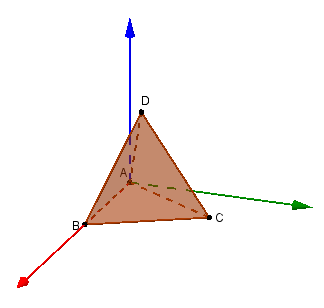
\includegraphics[width=0.5\textwidth]{02}
%%\end{figure}
%%
%%\ans
%%
%%\newpage
%%%
%%%\begin{figure}[h]
%%%\centering
%%%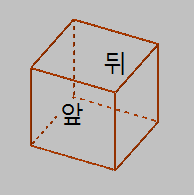
\includegraphics[width=0.5\textwidth]{a_cube}
%%%\end{figure}
%%
%%
%%\prob
%%한 모서리의 길이가 8cm이고 투명한 정육면체의 앞면과 뒷면에 각각 직사각형과 삼각형을 그린 후 색칠했습니다.
%%이 정육면체를 앞에서 볼 때, 색칠된 부분의 넓이를 구하시오.
%%
%%\begin{figure}[h]
%%\centering
%%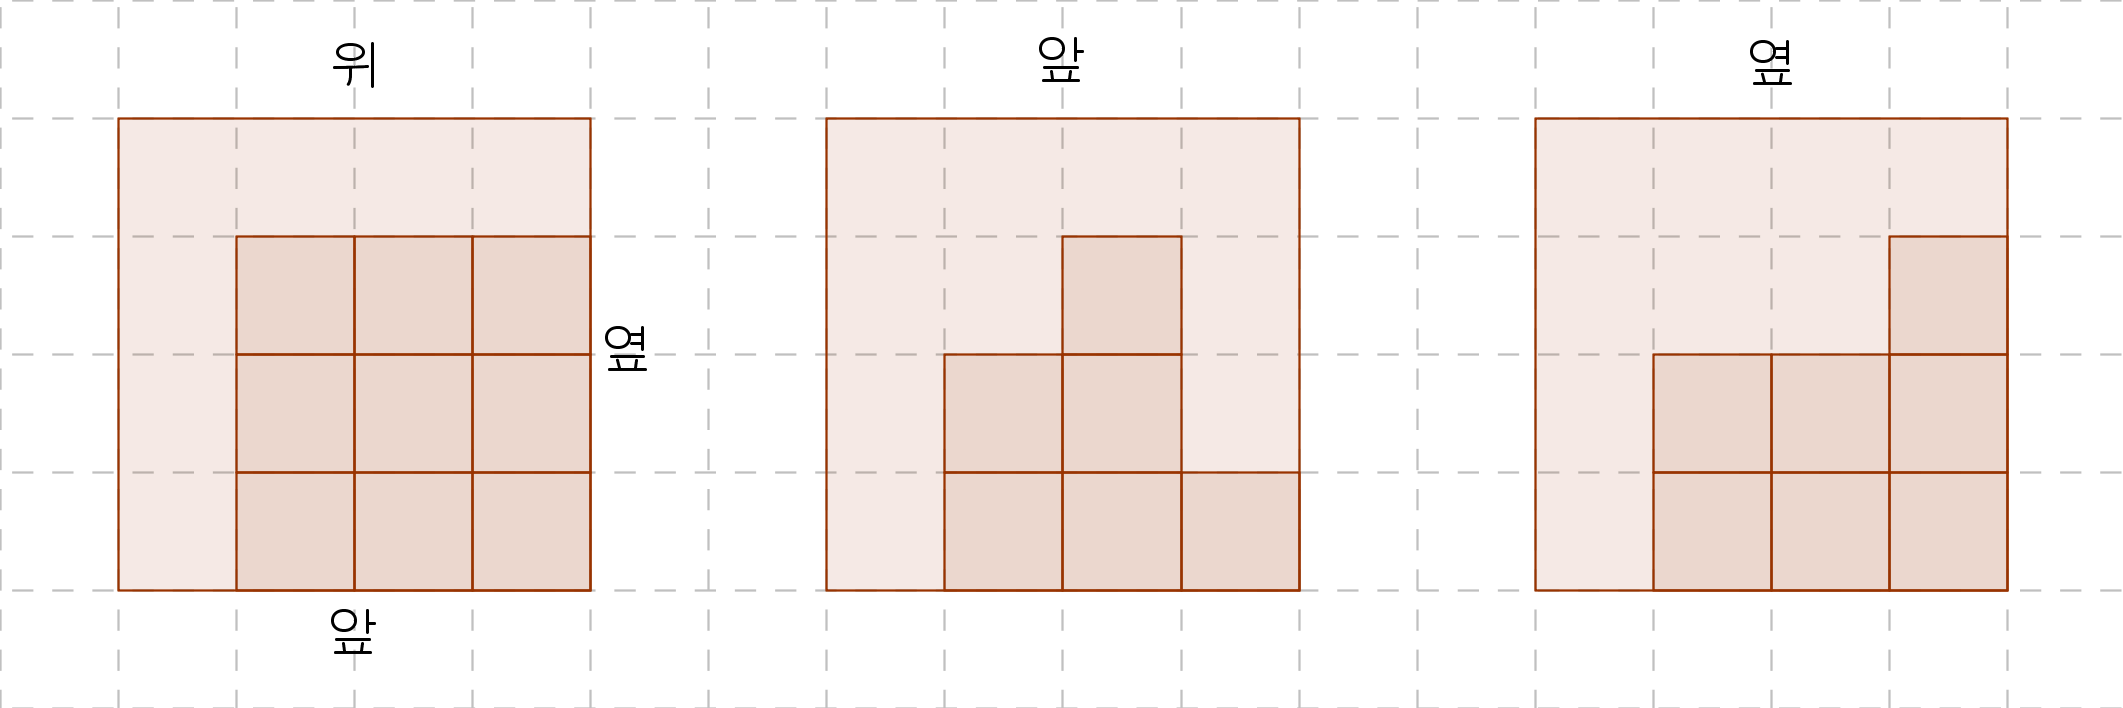
\includegraphics[width=\textwidth]{03}
%%\end{figure}
%%
%%\ans
%%
%%\prob
%%한 모서리의 길이가 6cm이고 투명한 정육면체의 앞면과 뒷면에 삼각형을 그린 후 색칠했습니다.
%%이 정육면체를 앞에서 볼 때, 색칠된 부분의 넓이를 구하시오.
%%
%%\begin{figure}[h]
%%\centering
%%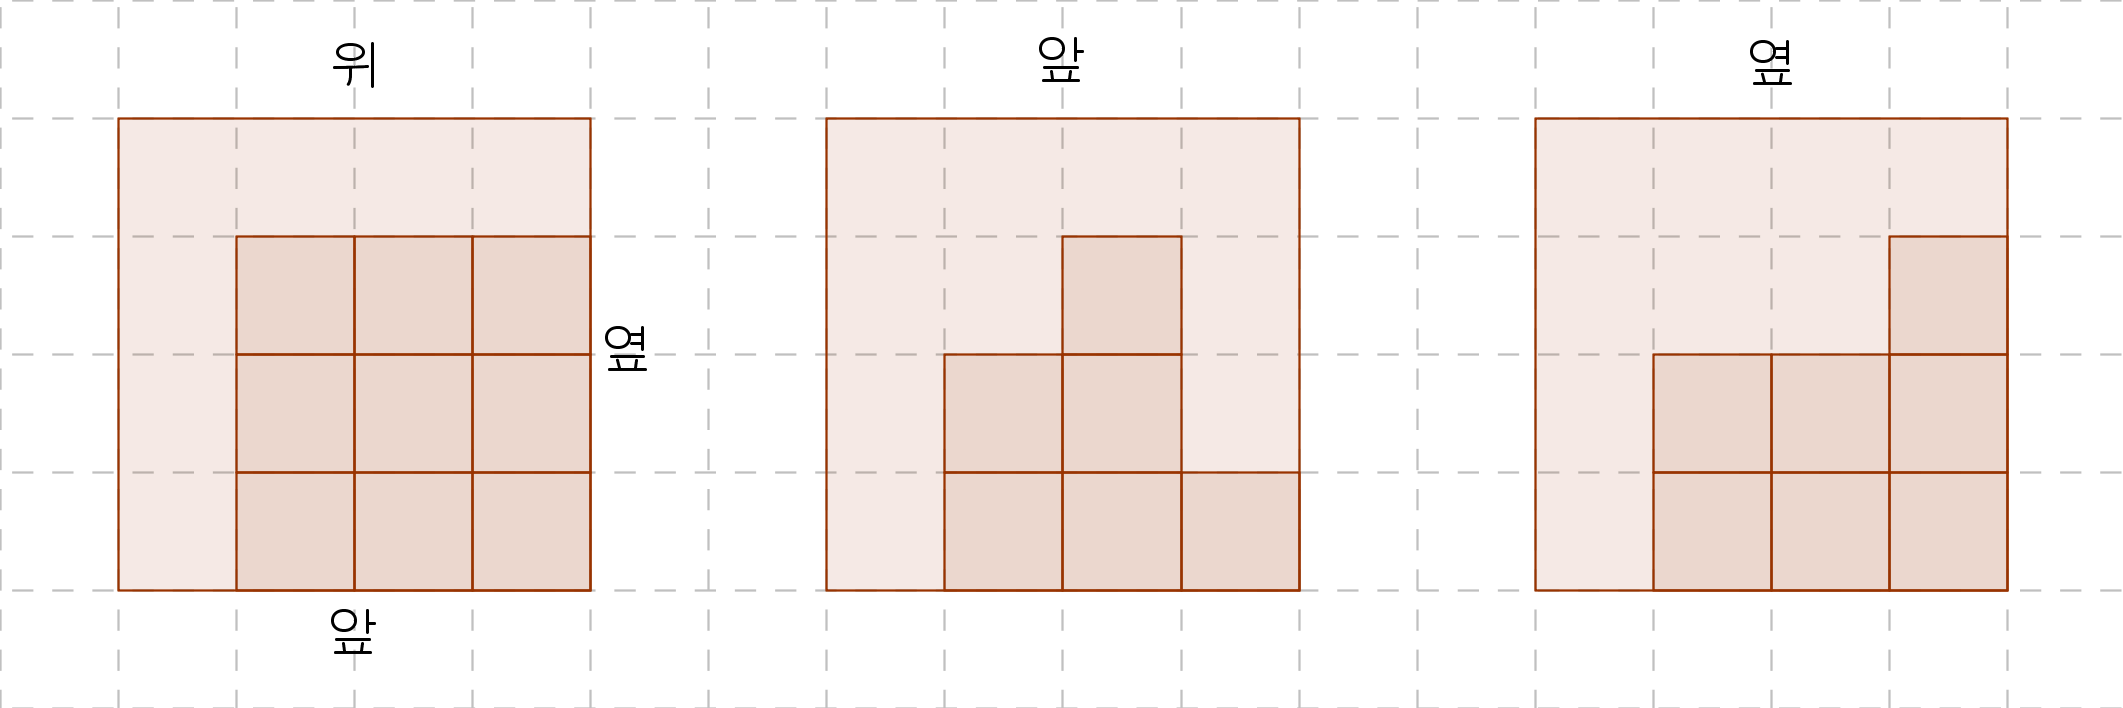
\includegraphics[width=\textwidth]{04}
%%\end{figure}
%%
%%\ans
%%
%%\newpage
%%
%%\prob
%%비 (가) : (나)를 가장 간단한 자연수의 비로 나타내어 보시오.
%%\[
%%\ga\times1\frac45=\na\times\frac74
%%\]
%%\ans
%%
%%\prob
%%비 (가) : (나)를 가장 간단한 자연수의 비로 나타내어 보시오.
%%\[
%%\ga\times2\frac32=\na\times1\frac14
%%\]
%%\ans
%%
%%\prob
%%비 (가) : (나)를 가장 간단한 자연수의 비로 나타내어 보시오.
%%\[
%%\ga\times\frac74=\na\times\frac{27}2
%%\]
%%\ans
%%
%%\prob
%%비 (가) : (나)를 가장 간단한 자연수의 비로 나타내어 보시오.
%%\[
%%\ga\times7\frac85=\na\times4\frac12
%%\]
%%\ans
%%
%%\newpage
%%
%%\prob
%%(가)의 0.45는 (나)의 \(\displaystyle\frac58\)과 같을 때 (가) : (나)를 가장 간단한 자연수의 비로 나타내어 보시오.
%%\begin{figure}[h]
%%\centering
%%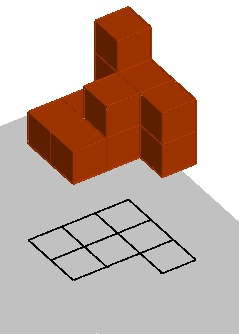
\includegraphics[width=0.5\textwidth]{09}
%%\end{figure}
%%
%%\ans
%%
%%\prob
%%(가)의 \(\displaystyle\frac5{16}\)는 (나)의 \(0.25\)과 같을 때 (가) : (나)를 가장 간단한 자연수의 비로 나타내어 보시오.
%%\begin{figure}[h]
%%\centering
%%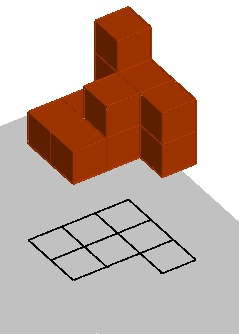
\includegraphics[width=0.5\textwidth]{09}
%%\end{figure}
%%
%%\ans
%%
%%\newpage
%%
%%(1km=1000m이고, 1m=100cm이며 1cm=10mm입니다.
%%이것을 이용하여 다음 문제들을 풀어보세요.)
%%
%%\prob
%%마라톤은 45.195km를 뛰는 운동경기입니다.
%%철수가 400m 둘레의 운동장을 35바퀴만큼 뛰었을 때, `철수가 달린 거리 : 마라톤 코스의 총 길이'를 가장 간단한 자연수의 비로 나타내세요.
%%\bigskip
%%
%%{\raggedleft\textbf{
%%철수가 달린 거리 : 마라톤 코스의 총 길이 = (\qquad\quad:\qquad\quad)}
%%\par}\bigskip\bigskip
%%
%%\prob
%%철수가 400m 둘레의 운동장을 몇 바퀴 돌아야 마라톤을 완주했다고 말할 수 있습니까?
%%
%%\ans
%%\begin{figure}[h]
%%\centering
%%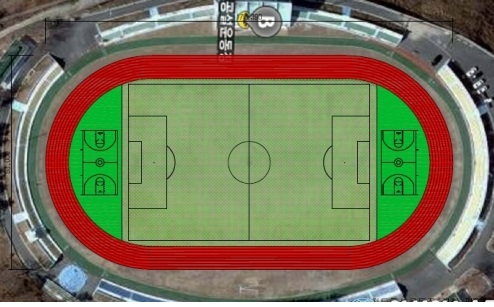
\includegraphics[width=0.7\textwidth]{track}
%%\end{figure}
%%
%%\newpage
%%
%%\prob
%%6.5mm길이의 일개미 400마리가 일렬로 늘어서 있습니다.
%%개미가 늘어선 길이와 몸길이가 4.5m인 악어의 길이의 비를 자연수의 비로 나타내세요.
%%(단, 개미 사이의 간격은 무시합니다.)
%%
%%{\raggedleft\textbf{
%%개미가 늘어선 길이 : 악어의 길이 = (\qquad\quad:\qquad\quad)}
%%\par}\bigskip\bigskip
%%
%%
%%\ans
%%\begin{figure}[h]
%%\centering
%%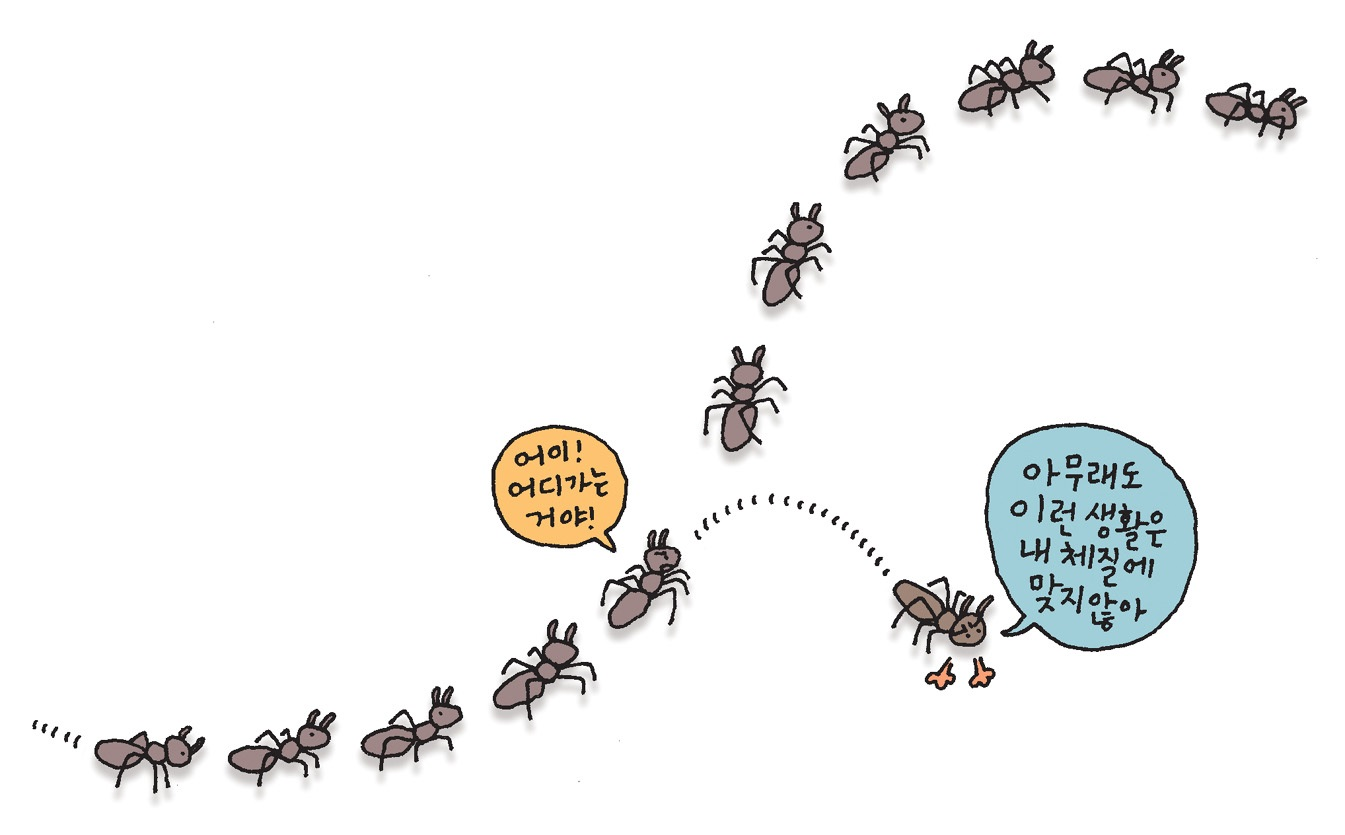
\includegraphics[width=0.7\textwidth]{ants}
%%\end{figure}
%%
%%\newpage
%%
%%\prob
%%고대 수학자인 탈레스는 피라미드 앞에 막대를 세워 놓고 피라미드의 그림자 길이와 막대의 그림자 길이를 잰 다음 비례식을 이용하여 거대한 피라미드의 높이를 재었습니다.
%%막대의 길이가 60cm, 막대의 그림자 길이가 130cm, 피라미드의 그림자의 길이가 5.2m일 때, 피라미드의 높이는 몇m인지 구하시오.
%%%{\center\small
%%%(막대 길이) : (막대의 그림자 길이) = (피라미드 높이) : (피라미드의 그림자 길이)
%%%}
%%
%%\ans
%%\begin{figure}[h]
%%\centering
%%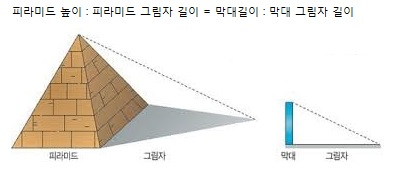
\includegraphics[width=0.8\textwidth]{pyramid}
%%\end{figure}
%%

\end{document}